\section{Components Implementation}

\subsection{Overview}

Chapter \ref{chapter:xbrl} introduced the concept of components in XBRL.
To recap, components act as chapters of a report and link together facts that belong to the same chapter.
In this chapter, we will look at how components are implemented in Brel.\cite{tesla_10q_2023_q3}
Brel closely follows the XBRL definition of components.\footnote{At the time of writing, the Open Information Model (OIM) does not define components.}
Throughout this chapter, we will use a running example to illustrate the concepts introduced in this chapter.

The XBRL specification uses the term "role" while Brel uses the term "component" to refer to the same concept. 

\subsection{Components in XBRL}

Components in XBRL are defined using the \texttt{link:roleType}\footnote{The prefix "link" commonly refers to the linkbase namespace 'http://xbrl.org/2003/linkbase'.} element. 
The following snippet shows an example of a component in XBRL:

\begin{figure}[H]
    \caption{Example of the component "Inventory" in XBRL from Tesla Inc.'s 2023 Q3 report\cite{tesla_10q_2023_q3}}
    \label{fig:example_component_xbrl}
    % make the text size smaller
    \begin{lstlisting}[language=XML,basicstyle=\fontsize{7}{10}\selectfont\ttfamily]
      <link:roleType id="Inventory" roleURI="http://www.tesla.com/role/Inventory">
        <link:definition>0000010 - Disclosure - Inventory</link:definition>
        <link:usedOn>link:presentationLink</link:usedOn>
        <link:usedOn>link:calculationLink</link:usedOn>
        <link:usedOn>link:definitionLink</link:usedOn>
      </link:roleType>
    \end{lstlisting}
\end{figure}

I will refer to the component in figure \ref{fig:example_component_xbrl} as the "Inventory" component.
All properties of XBRL components are either required or optional.
I will use the notation \texttt{(required)} and \texttt{(optional)} to indicate the requiredness of a property.
The Inventory component has the following properties:

\begin{itemize}
  \item \texttt{roleURI} (required): The URI of the Inventory component. This URI is used to reference the component from other elements in the XBRL taxonomy. It is the primary identifier of the component. 
  The roleURI has to be unique on a per-taxonomy basis.\cite{xbrl21_custom_roles}
  \item \texttt{id} (optional): The id of the component, which is commonly used to reference the component from other elements in the XBRL report.
  \footnote{Even though the id is optional, it is recommended to provide an id for each component.\cite{xbrl21_custom_roles}}
  \footnote{Similar to the roleURI, the id has to be unique on a per-taxonomy basis.\cite{xml_id}}
  \item \texttt{definition} (optional): A human-readable description of the component. 
  \item \texttt{usedOn}: A list of links that the component is used in. 
  Whenever a link uses a component, it must declare the component in the \texttt{usedOn} property.
  \footnote{The \texttt{usedOn} property is only required for standard extended links and standard resource elements.\cite{xbrl21_custom_roles}}
  Therefore, the \texttt{usedOn} property can be interpreted as a list of possible links that can use the component.
  However, even though the Invenory component indicates the use of e.g. a presentation link, it does not mean that any presentation ;oml is defined for the component.
\end{itemize}

Most of the roles in XBRL will not be defined by the creators of the report, but rather by the creators of the XBRL taxonomy. 
In the case of Tesla Inc.'s 2023 Q3 report, only 60 components are defined by the creators of the report, while roughly 600 components are defined by the creators of the XBRL taxonomy.\cite{tesla_10q_2023_q3}

\subsection{Components in Brel}

The main difference between components in XBRL and Brel is that Brel abstracts away the \texttt{usedOn} property. 
Instead, components in Brel provide a direct way of accessing the links that use the component. 
A component in Brel is defined using the \texttt{Component} class. 
The following UML diagram shows the class diagram of the \texttt{Component} class:

\begin{figure}[H]
  \caption{UML diagram of the \texttt{Component} class}
  \label{fig:uml_component}
  \centering
  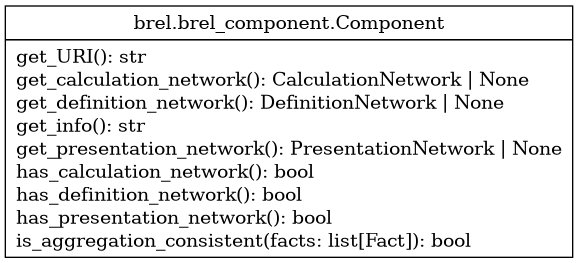
\includegraphics[width=0.8\textwidth]{images/brel.brel_component.Component.png}
\end{figure}

% The \texttt{get\_info} method refers to the text of the definintion element in the XBRL taxonomy.
The \texttt{get\_info} method returns the text of the definition element if it exists, otherwise it returns \texttt{None}.
This renaming was done to avoid confusion with the \texttt{get\_definition\_network} method that returns the definition network of the component.

The \texttt{get\_URI} method returns the URI of the role of the component.

Even though the \texttt{usedOn} property has been discarded, during parsing, Brel will still perform a check for the \texttt{usedOn} property.
More precisely, if there exists a non-standard network that is associated with the component, Brel will check if the \texttt{usedOn} property is defined for the component.
If not, Brel will raise an exception.

The three methods \texttt{get\_presentation\_network}, \texttt{get\_calculation\_network}, and \texttt{get\_definition\_network} return the respective networks of the component.
They return \texttt{None} if the network in question does not exist for the component.

Using the three methods \texttt{has\_presentation\_network}, \texttt{has\_calculation\_network}, and \texttt{has\_definition\_network}, it is possible to check if the respective network exists for the component.

Finally, the \texttt{sums\_up} method acts as a shortcut for the \texttt{sums\_up} of the calculation network of the component.
If the component does not have a calculation network, the \texttt{sums\_up} method will return \texttt{True}.


